% Uncomment the following line if the paper is going to be published in journal

%\documentclass[journal, twoside]{IEEEtran}

% Uncomment the following line if the paper is going to be published on the conference

\documentclass[conference]{IEEEtran}

% Warning: different journals/conferences migh have different requirements for the papers this is just a default template

%*********************************************************************************************************************************

% Importing packages -  beginning

\IEEEoverridecommandlockouts
% The preceding line is only needed to identify funding in the first footnote. If that is unneeded, please comment it out.
\usepackage{cite}
\usepackage{amssymb,amsfonts}
\usepackage{amsmath}
\interdisplaylinepenalty=2500
\usepackage{algorithmic}
\usepackage{graphicx}
\usepackage{textcomp}
\usepackage{xcolor}
\def\BibTeX{{\rm B\kern-.05em{\sc i\kern-.025em b}\kern-.08em
		T\kern-.1667em\lower.7ex\hbox{E}\kern-.125emX}}	


\makeatletter
\def\endthebibliography{%
	\def\@noitemerr{\@latex@warning{Empty `thebibliography' environment}}%
	\endlist
}
\makeatother

\renewcommand{\encodingdefault}{OT1}
\usepackage[utf8]{luainputenc}

\usepackage[withpage, nohyperlinks]{acronym}

\usepackage[spaces,hyphens]{xurl} % allow arbitrary line breaks in a formatted URL string
\usepackage[colorlinks,allcolors=blue]{hyperref}
\usepackage{caption}
%\usepackage{glossaries-extra}

% Importing packages - end

%*********************************************************************************************************************************


\begin{document}
	\urlstyle{tt}
	
	\title{Template for IEEE Papers}
	
	\ifCLASSOPTIONconference
		% You must choose one of three types of author names format when using conference paper
		% alternate form to use when authors are from the same organization

\author{
	\IEEEauthorblockN{
				Batman\IEEEauthorrefmark{1}, 
				Homer Simpson\IEEEauthorrefmark{1}, 
				and Joker\IEEEauthorrefmark{1},
			}
	
	\IEEEauthorblockA{
				\IEEEauthorrefmark{1}
				Department of Technical Cybernetics\\
				Faculty of Management Science and Informatics\\
				University of Žilina\\
				Slovakia, Žilina\\				
				Email:
				\href{mailto:batman@fri.uniza.sk}{batman@fri.uniza.sk}, \href{mailto:homer.simpson@fri.uniza.sk}{homer.simpson@fri.uniza.sk}, \href{mailto:joker@fri.uniza.sk}{joker@fri.uniza.sk},   
			}

}
	
	

%% For less than 4 authors
%
%\author{
%	\IEEEauthorblockN{
%		Michael Shell
%	}
%	
%	\IEEEauthorblockA{
%		School of Electrical and\\
%		Computer Engineering\\
%		Georgia Institute of Technology\\
%		Atlanta, Georgia 30332--0250\\
%		Email: mshell@ece.gatech.edu
%	}
%	
%	\and
%	
%	\IEEEauthorblockN{
%		Homer Simpson
%	}
%	
%	\IEEEauthorblockA{
%		Twentieth Century Fox\\
%		Springfield, USA\\
%		Email: homer@thesimpsons.com
%	}
%	
%	\and
%	
%	\IEEEauthorblockN{James Kirk\\
%		and Montgomery Scott
%	}
%	
%	\IEEEauthorblockA{
%		Starfleet Academy\\
%		San Francisco, California 96678-2391\\
%		Telephone: (800) 555--1212\\
%		Fax: (888) 555--1212
%	}
%			
%}



%% For more than 3 authors
%
%\author{
%	
%	\IEEEauthorblockN{
%		Michael Shell\IEEEauthorrefmark{1}, 
%		Homer Simpson\IEEEauthorrefmark{2}, 
%		James Kirk\IEEEauthorrefmark{3},
%		Montgomery Scott\IEEEauthorrefmark{4}
%		and Eldon Tyrell\IEEEauthorrefmark{1}
%	}
%	
%	\IEEEauthorblockA{
%		\IEEEauthorrefmark{1}
%		School of Electrical and Computer Engineering\\
%		Georgia Institute of Technology, Atlanta, Georgia 30332--0250\\
%		Email: mshell@ece.gatech.edu
%	}
%	
%	\IEEEauthorblockA{
%		\IEEEauthorrefmark{2}
%		Twentieth Century Fox, Springfield, USA\\
%		Email: homer@thesimpsons.com
%	}
%
%	\IEEEauthorblockA{
%		\IEEEauthorrefmark{3}
%		Starfleet Academy, San Francisco, California 96678-2391\\
%		Telephone: (800) 555--1212, Fax: (888) 555--1212
%	}
%	
%	\IEEEauthorblockA{
%		\IEEEauthorrefmark{4}
%		Tyrell Inc., 123 Replicant Street, Los Angeles, California 90210--4321
%	}
%			
%}

	\else
		\author{
	Batman,
	\IEEEmembership{Member, IEEE,} 
	Homer Simpson,
	\IEEEmembership{Fellow, OSA,}
	and Joker,
	\IEEEmembership{Life Fellow, IEEE}
	
}
	\fi	
	
	\ifCLASSOPTIONjournal
		\markboth
		{Journal of Quantum Telecommunications, Vol. 1, No. 1, January 2100}
		% The second argument is used as a page heading only for the odd number pages after the title page for two sided (duplex) journal papers,
		{\MakeLowercase{Template for IEEE Papers, University of Žilina, Faculty of Management Science and Informatics}}
	\fi
	
	
	\ifCLASSOPTIONjournal
		\IEEEpubid{0000--0000/00\$00.00~\copyright~2024 IEEE}
		% Remember, if you use \IEEEpubid you must call \IEEEpubidadjcol in the second and first
		% column for its text to clear the IEEEpubid mark.
	\fi
	
	% In journal mode command causes error
	%\IEEEspecialpapernotice{(Template paper)}

	\maketitle	

	
	\begin{abstract}
	Here you write abstract.
\end{abstract}

\begin{IEEEkeywords}
	Here you write key words.
\end{IEEEkeywords}
	
	%Glossary
	\section*{List of Acronyms}

% With the following command we can add padding between acronym and its meaning
\renewcommand{\IEEEiedlistdecl}{\IEEEsetlabelwidth{SONET}}

\begin{acronym}
	\hypersetup{hidelinks}
	
	\acro{ram}[RAM]{Random Access Memory}
	\acro{fri}[FRI]{Faculty of Management Science and Informatics}
	\acro{iot}[IoT]{Internet-of-Things}
	
	\acrodefplural{iot}[IoTs]{Internets-of-Things}
	
\end{acronym}

\renewcommand{\IEEEiedlistdecl}{\relax} %reset back
	

	% Remember, if you use \IEEEpubid you must call \IEEEpubidadjcol in the second and first
	% column for its text to clear the IEEEpubid mark.
	\IEEEpubidadjcol
	
	
	
	\section{INTRODUCTION}

This is the introduction of the paper.
	
	% Add here the sections of your conference paper - beginning
	
	\section{MY ONLY SECTION}

	\ifCLASSOPTIONjournal
		\IEEEPARstart{J}{urnals} use this convention for the first letter of a journal paper.
	\else
		Conference papers use normal size for the first letter of the conference paper.
	\fi	

The \ac{iot} is becoming very popular. One of the elements of \ac{iot} are embedded systems. There is a lot of \aclp{iot} devices currently on the market the acronym for them is \acsp{iot}.

On the \acf{fri} you will learn about \acs{ram} which is short for \acl{ram}.

The monkeys are very smart animals \cite{article_first}. They are shown in \figurename ~\ref{fig:monkey}. 

\begin{figure}[ht]
	\centering
	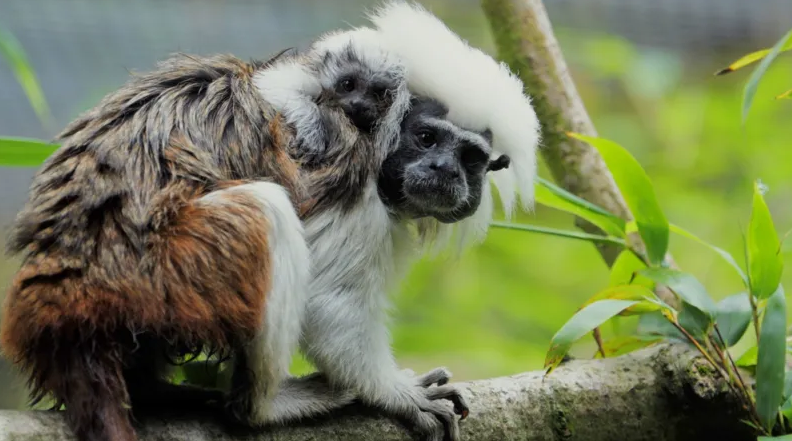
\includegraphics[width=1.0\linewidth]{pictures/monkey}
	\caption{Nice picture of monkey \cite{figure_first}}
	\label{fig:monkey}
\end{figure}


We can use vibrational energy harvesting during monkey studies \cite{article_second}. Its basic principle is shown in \figurename  ~\ref{fig:vibrationalenergyharvesting}.

\begin{figure}[ht]
	\centering
	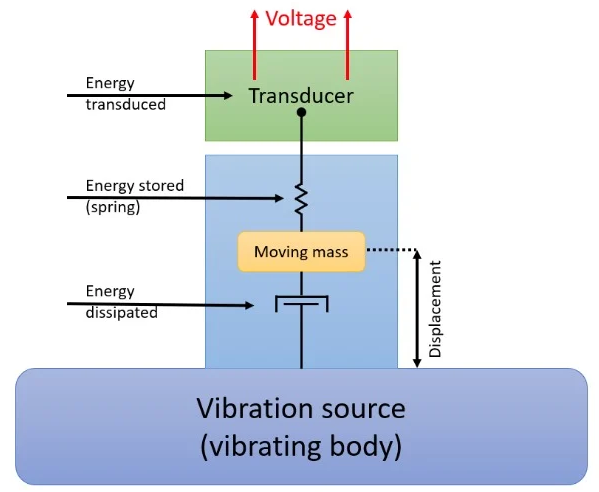
\includegraphics[width=1.0\linewidth]{pictures/vibrational_energy_harvesting}
	\caption{Vibrational energy harvesting principle \cite{figure_second}}
	\label{fig:vibrationalenergyharvesting}
\end{figure}

This is how you should cite text that has multiple sources \cite{article_first, article_second}.

In table \ref{tab:first_table} we have some measured data.

\begin{table}[ht]
	\centering
	\caption{My first table}
	\label{tab:first_table}
	\begin{tabular}{|c|c|c|c|}
		\hline
		& $a$ & $b$ & $c$ \\
		\hline
		$a$ & 1 & 0 & 1 \\
		\hline
		$b$ & 0 & 1 & 1 \\
		\hline
		$c$ & 1 & 1 & 0 \\
		\hline
	\end{tabular}
\end{table}

And in the \eqref{eq:original_equation} is shown a very simple formula. Based on which the variable $a$ is a sum of two variables $b$ and $c$.

\begin{equation}
	\label{eq:original_equation}
	a = b + c
\end{equation}

We can also calculate the value of variable $c$ by altering the equation as in \eqref{eq:altered_equation}. 

\begin{equation}
	\label{eq:altered_equation}
	c = a - b
\end{equation}


% When using journal as document class do the following
% Remember, if you use \IEEEpubid you must call \IEEEpubidadjcol in the second and first
% column for its text to clear the IEEEpubid mark.
\IEEEpubidadjcol

This way we can create a plain unnumbered list.

\begin{list}{}{}
	\item Hope
	\item Elizabeth
	\item Josette 
\end{list}

This way we can create an unnumbered list.

\begin{itemize}
	\item Hope
	\item Elizabeth
	\item Josette
\end{itemize}

This way we can create an numbered list.

\begin{enumerate} 
	\item Hope
	\item Elizabeth
	\item Josette
\end{enumerate}

This way we can create lists with descriptions.

\begin{description}
	\item[red] nice colour
	\item[blue] not very nice colour
\end{description}


	
	
	% Add here the sections of your conference paper - end
	
	
	\section{CONCLUSION}

This is the conclusion of the paper.

	
	
	
	\section*{Acknowledgment}

The authors would like to thank...
	
	
	
	% If you are using TexStudiu you have to choose Tools → Commands → Bibtex and then recompile to sort the references based on their order of citations in the document.
	% You can also add shortcut for Bibtex to the upper menu. Based on pictures from the folder bibliography_recompilation_guide. 
	
	% If you are using Overleaf then it will automatically sort the references for you.
	\nocite{*}
	\bibliographystyle{IEEEtran}
	\bibliography{IEEEabrv,./bibliography/refs.bib}
	
	\ifCLASSOPTIONjournal
		\vskip 0pt plus -1fil
\begin{IEEEbiographynophoto}
	{Batman}

	I am the author of this IEEE template. And I don't like pictures.
	
\end{IEEEbiographynophoto}

\vskip 0pt plus -1fil
\begin{IEEEbiography}
	% Source: https://www.onthisday.com/people/homer-simpson
	[{
\includegraphics[width=1in,height=1.25in,clip,keepaspectratio]{./biographies/homer_simpson.jpg}}]	
	{Homer Simpson}
	
	I like steaks and bear.
	
\end{IEEEbiography}

\vskip 0pt plus -1fil
\begin{IEEEbiography}
	% Source: https://www.pinterest.com/pin/joker-by-bruce-timm--505810601898941193/
	[{
\includegraphics[width=1in,height=1.25in,clip,keepaspectratio]{./biographies/joker.jpg}}]	
	{Joker}
	
	I am the biggest enemy of the batman.
	
\end{IEEEbiography}
	\fi
	
	
	
\end{document}

\begin{comment}
	
% If you don't know what to put to certain fields don't erase them just leave them empty they will be automatically ignored when the references are generated.

% Template for articles in biblography

@article{,
	title        = {},
	author       = {},
	year         = {},
	month        = {},
	journal      = {},
	booktitle    = {},
	volume       = {},
	number       = {},
	pages        = {},
	doi          = {},
	issn         = {},
	url          = {},
}

% Example usage 

@article{vibrations,
	title        = {A study of low level vibrations as a power source for wireless sensor nodes},
	author       = {Shad Roundy and Paul K. Wright and Jan Rabaey},
	year         = {2003},
	month        = {July},
	journal      = {Computer Communications},
	booktitle    = {},
	volume       = {26},
	number       = {11},
	pages        = {1131--1144},
	doi          = {https://doi.org/10.1016/S0140-3664(02)00248-7},
	issn         = {0140-3664},
	url          = {https://www.sciencedirect.com/science/article/pii/S0140366402002487},
}

% Template for Figures in biblography

@online{,
	title        = {},
	author       = {},
	url          = {},
	year         = {},
}


% Example usage

@online{monkeys,
	title        = {Introduction to Vibration Energy Harvesting},
	author       = {Francesco Orfei},
	url          = {https://www.allaboutcircuits.com/technical-articles/introduction-to-vibration-energy-harvesting/},
	year         = {2019},
}

\end{comment}
